\subsection{Proving the general theroem}
\label{sub:Proving the general theroem}
We will now look at the general version of our theorem, where the set of nodes $Y$ can contain any number of nodes\todo{is infinite neccessary here?}.  We thus have the following situation:
\[
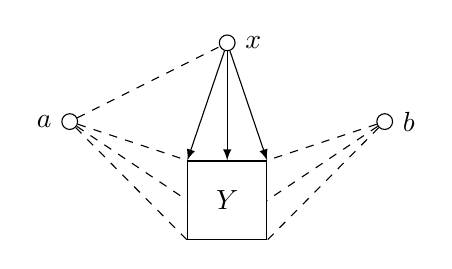
\begin{tikzpicture}
  [
  point/.style={circle,draw,inner sep=0pt,minimum size=2mm},
  set/.style={rectangle,draw,inner sep=0pt,minimum size=10mm}
  ]
  \node (a) at (0,1) [point,label=left:$a$] {};
  \node (b) at (4,1) [point,label=right:$b$] {};

  \node (x) at (2,2) [point,label=right:$x$] {};
  \node (y) at (2,0) [set,label=center:$Y$] {};

  \draw [-latex] (x) to (y.north);
  \draw [-latex] (x) to (y.north west);
  \draw [-latex] (x) to (y.north east);
  \draw [dashed] (a) to (x);
  \draw [dashed] (a) to (y.west);
  \draw [dashed] (a) to (y.south west);
  \draw [dashed] (a) to (y.north west);
  \draw [dashed] (b) to (y.east);
  \draw [dashed] (b) to (y.north east);
  \draw [dashed] (b) to (y.south east);
\end{tikzpicture}
\]
As earlier, arrows represent edges, while dashed lines represents vels.
$Y$ is now a set of nodes in which all elements are targeted by an edge from $x$ and a vel from either $a$ or $b$.

Using our notation, we get the following statement:
\begin{align*}
  E(x,Y),V(a,x),\bigwedge_{y \in Y}V(a,y){\vee V(b,y)}
\end{align*}
As we discovered earlier, whether an element in $Y$ is connected by a vel to $a$ or $b$ does not really matter for the proof.
Therefore, in order to reduce the number of cases to prove, we will enumerate the elements in $Y$ and let $v_i \in \{a,b\}$ denote the node connceted to $y_i \in Y$. By doing this, we get a simpler statement, both visually and with respect to the upcomming proof.  We now have the following statement (with $y_i \in Y$):
\begin{align*}
  E(x,Y),V(a,x),V(v_1,y_1),V(v_2,y_2),\dots,V(v_n,y_n)
\end{align*}
We will now expand this statement using our vel definition.  Using the general definiton of vels, we will not get $2^n$ different cases, but we still want to distinguish between the two cases we get from $V(a,x)$.  Our two cases are therefore:
\begin{enumerate}[(i)]
  \item $E(x,Y),\poo(a,c_0),\poe(x,c_0),\p o {\lambda_1}(v_1,c_1),\p o {\overline{\lambda_1}}(y_1,c_1), \dots, \p o {\lambda_n}(v_n,c_n),\p o {\overline{\lambda_n}}(y_n,c_n)$
  \item $E(x,Y),\poe(a,c_0),\poo(x,c_0),\p o {\lambda_1}(v_1,c_1),\p o {\overline{\lambda_1}}(y_1,c_1), \dots, \p o {\lambda_n}(v_n,c_n),\p o {\overline{\lambda_n}}(y_n,c_n)$
\end{enumerate}
\subsubsection{Proof, case i}
\label{subs:Proof, case i}
\begin{prooftree*}[downwards]
  \Hypo{V_o(a,b)}
  \Infer1[def]{\ax{\pox(b,d)},\ponx(a,d)}
  \Infer1[GC1]{\ax{\poo(a,c)},\pex(c,d)}
  \Infer1[GC2]{\ax{\ponx(y,d)},P^f_o(c,y)}
  \Infer1[L3]{E(c,\{y\})}
  \Infer1[(=)]{\ax{E(x,\{y\})}, x=c}
  \Hypo{V_o(a,b)}
  \Infer1[def]{\ax{\pox(b,d)},\ponx(a,d)}
  \Infer1[GC1]{\ax{\poo(a,c)},\pex(c,d)}
  \Hypo{V_o(a,b)}
  \Infer1[def]{\ax{\poo(a,c)},\poe(b,c)}
  \Infer1[GC1]{\ax{\pox(b,d)}\p xx(d,c)}
  \Infer2[GB3]{\peo(y,c),\ax{\ponx(y,d)}}
  \Infer2[S3]{\ax{\poe(x,c)},\ax{E(x,\{y\})}}
\end{prooftree*}
